\documentclass[13pt, a4paper]{article}
\usepackage[utf8]{vietnam} 
\usepackage{amssymb,gensymb,textcomp} \usepackage{array,multicol,multirow,siunitx,tabularx}
\usepackage{graphicx} 
\usepackage{float}
\usepackage{multicol}
\usepackage{multirow}
\usepackage{adjustbox}
\usepackage{lipsum}
\usepackage{subcaption}
\usepackage{enumerate}
\usepackage{indentfirst}
\usepackage{amsmath} 
\usepackage{listings}
\usepackage{diagbox}
\usepackage{matlab-prettifier}
\usepackage{xcolor}
\usepackage{color}
\definecolor{light-gray}{gray}{0.95}
\newcommand{\code}[1]{\colorbox{light-gray}{\texttt{#1}}}
\usepackage{titlesec}
\usepackage{amsfonts} 
\usepackage{caption}
\usepackage{subcaption}
\usepackage{amssymb} 
\usepackage{rotating}
\usepackage{tikz}
\usepackage[colorlinks = true,
            linkcolor = black,
            urlcolor  = blue,
            citecolor = blue,
            anchorcolor = blue]{hyperref}
\usepackage{enumitem}
\usepackage[left=2.3cm,right=2cm,top=2.5cm,bottom=2.5cm]{geometry} 
\usepackage{scrextend}
\usepackage{algorithm2e}
\usepackage{etoolbox}
\usepackage{ragged2e}
\usepackage{minted}
\usepackage{lastpage}
\changefontsizes[23pt]{13pt}
\usepackage{fancyhdr}
\usepackage{tikz,tkz-tab}
\usetikzlibrary{shapes.geometric, arrows}
\usepackage[framemethod=TikZ]{mdframed}
\usepackage{amsthm}
\usepackage{xurl}
\usepackage{commath}
\usepackage{framed}
\usepackage{commath}
\usepackage{framed}
\usepackage{enumitem}
\usepackage{booktabs}
\makeatletter
\newcommand{\mylabel}[2]{#2\def\@currentlabel{#2}\label{#1}}
\makeatother


\renewcommand{\figureautorefname}{Hình}
\renewcommand{\tableautorefname}{Bảng}
\renewcommand{\equationautorefname}{Phương trình}
\renewcommand{\sectionautorefname}{Mục}
\renewcommand{\subsectionautorefname}{Phần}
\renewcommand{\subsubsectionautorefname}{Phần}
\renewcommand{\itemautorefname}{}
\setlength{\headheight}{20pt}
\captionsetup{labelfont={bf}}
\pagestyle{fancy}

\fancyhf{} % clear all header fields
\fancyhead[L]{
 \begin{tabular}{rl}
    \begin{picture}(15,15)(0,0)
    \put(0,-8){
\includegraphics[width=8.7mm, height=8.7mm]{picture/01_logobachkhoasang.png}}
   \end{picture}&
	\begin{tabular}{l}
		\textbf{\bf \ttfamily Trường Đại học Bách khoa - ĐHQG–HCM}
             \\[-1.4ex] \textbf{\bf \ttfamily Khoa Khoa học và Kỹ thuật Máy tính}
	\end{tabular} 
 \end{tabular}
}
\fancyhead[R]{
 \begin{tabular}{r}
    \textbf{\bf \ttfamily Nhóm 7} % header
\end{tabular}
}
\fancyfoot{} % clear all footer fields
\fancyfoot[L]{\footnotesize \ttfamily {Bài tập lớn 1 Hệ cơ sở dữ liệu - HK251}} % footer 
\fancyfoot[R]{\footnotesize \ttfamily {Trang {\thepage}/{\hypersetup{}\pageref{LastPage}}}}

\renewcommand{\footrulewidth}{1pt}
\definecolor{codegreen}{rgb}{0,0.6,0}
\definecolor{codegray}{rgb}{0.5,0.5,0.5}
\definecolor{codepurple}{rgb}{0.58,0,0.82}
\definecolor{backcolour}{rgb}{0.95,0.95,0.92}

\lstdefinestyle{mystyle}{
    language=R,% set programming language
    backgroundcolor=\color{backcolour},   
    commentstyle=\color{codegreen},
    keywordstyle=\color{blue},
    numberstyle=\tiny\color{codegray},
    stringstyle=\color{codepurple},
    basicstyle=\ttfamily\footnotesize,
    breakatwhitespace=false,         
    breaklines=true,
    captionpos=b,                    
    keepspaces=true,                 
    numbers=left,                    
    numbersep=5pt,
    frame = tb,
    showspaces=false,                
    showstringspaces=false,
    showtabs=false,                  
    tabsize=2
    escapeinside={(*}{*)},% escaping to LaTeX
    fancyvrb=true,% verbatim code is typset by listings
    extendedchars=false,% prohibit extended chars (chars of codes 128--255)
    alsoother={\$},% becomes other
    otherkeywords={!=, \~, \$, \&, \%/\%, \%*\%, \%\%, <-, <<-, /},% other keywords
    deletekeywords={c}% remove keywords
}

\usepackage{bashful}
\usepackage{tcolorbox}
\tcbuselibrary{minted,breakable,xparse,skins}
\definecolor{bg}{gray}{0.95}
\DeclareTCBListing{mintedbox}{O{}m!O{}}{%
  breakable=true,
  listing engine=minted,
  listing only,
  minted language=#2,
  minted style=default,
  minted options={%
    linenos=true,
    gobble=0,
    breaklines=true,
    breakafter=,,
    fontsize=\small,
    numbersep=8pt,
    #1},
  boxsep=0pt,
  left skip=0pt,
  right skip=0pt,
  left=25pt,
  right=0pt,
  top=3pt,
  bottom=3pt,
  arc=5pt,
  leftrule=0pt,
  rightrule=0pt,
  bottomrule=2pt,
  toprule=2pt,
  colframe=black!100,
  enhanced,
  overlay={%
    \begin{tcbclipinterior}
    \fill[lightgray] (frame.south west) rectangle ([xshift=20pt]frame.north west);
    \end{tcbclipinterior}},
  #3}

\makeatletter
\AtBeginEnvironment{mintedbox}{\dontdofcolorbox}
\def\dontdofcolorbox{\renewcommand\fcolorbox[4][]{##4}}
\makeatother

\setcounter{secnumdepth}{4}

\titleformat{\paragraph}
{\normalfont\normalsize\itshape}{\theparagraph}{1em}{}
\titlespacing*{\paragraph}
{0pt}{3.25ex plus 1ex minus .2ex}{1.5ex plus .2ex}
\begin{document}

\include{content/Bìa} 
\tableofcontents 
\section{Giới thiệu}
Trong kỷ nguyên chuyển đổi số hiện nay, việc học lập trình trực tuyến đã trở thành xu hướng tất yếu và ngày càng khẳng định vai trò quan trọng trong việc đào tạo nguồn nhân lực công nghệ chất lượng cao. Lấy cảm hứng từ nền tảng CodeLearn, hệ thống E-Learning Coding được thiết kế như một môi trường học lập trình toàn diện, nơi người học có thể tiếp cận kiến thức từ cơ bản đến nâng cao một cách có hệ thống và hiệu quả.

Hệ thống E-Learning Coding hướng đến việc xây dựng một cộng đồng học lập trình sôi động, nơi các giảng viên có thể dễ dàng xây dựng và quản lý các khóa học lập trình chất lượng, từ các ngôn ngữ cơ bản như HTML, CSS, JavaScript đến các framework hiện đại và các kỹ thuật lập trình nâng cao. Mỗi khóa học được thiết kế với lộ trình rõ ràng, kết hợp hài hòa giữa lý thuyết và thực hành, giúp người học không chỉ nắm vững kiến thức mà còn phát triển kỹ năng giải quyết vấn đề thông qua hàng trăm bài tập coding thực tế.

Điểm khác biệt của hệ thống là tích hợp sẵn môi trường thực hành coding trực tuyến, cho phép người học viết, chạy và kiểm tra code ngay trên trình duyệt mà không cần cài đặt bất kỳ công cụ nào. Hệ thống tự động chấm điểm và đánh giá code của người học, cung cấp phản hồi tức thì về hiệu suất và chất lượng code. Bên cạnh đó, tính năng theo dõi tiến độ học tập chi tiết giúp người học nhận biết được điểm mạnh, điểm yếu và có kế hoạch học tập phù hợp.

Hệ thống cũng chú trọng xây dựng cộng đồng học tập tương tác cao thông qua diễn đàn thảo luận, nơi người học có thể trao đổi kiến thức, chia sẻ kinh nghiệm giải quyết các bài tập khó, và nhận được sự hỗ trợ kịp thời từ giảng viên và bạn học. Các tính năng của hệ thống giúp tạo động lực học tập và khuyến khích tinh thần cạnh tranh lành mạnh.

Với đội ngũ giảng viên giàu kinh nghiệm và hệ thống nội dung được cập nhật liên tục theo xu hướng công nghệ mới nhất, E-Learning Coding hướng đến mục tiêu trở thành nền tảng đào tạo lập trình trực tuyến hàng đầu, cung cấp cho người học những kỹ năng lập trình thực tiễn và cần thiết để thành công trong sự nghiệp công nghệ.



\section{Phân tích và mô tả yêu cầu dữ liệu}
\subsection{Tìm hiểu ứng dụng hoặc hệ thống liên quan}
%TODO
Tên hệ thống: \textbf{CodeLearn} - Nền tảng học tập trực tuyến.

Đường dẫn: \url{https://codelearn.io}

Phân tích nghiệp vụ chính của hệ thống: Hệ thống CodeLearn vận hành với nhiều nghiệp vụ chính. Trước hết, người dùng có thể đăng ký tài khoản bằng email hoặc mạng xã hội, sau đó truy cập hồ sơ cá nhân để theo dõi lịch sử học tập và tiến độ từng khóa học. Mỗi khóa học bao gồm nhiều chương và bài học, có thể ở dạng lý thuyết, video hoặc bài tập lập trình trực tiếp trên trình duyệt. Hệ thống tự động chấm điểm các bài tập dựa trên bộ test công khai và ẩn, trả về kết quả chi tiết về độ chính xác, thời gian và bộ nhớ sử dụng. Khi hoàn thành tối thiểu 80\% nội dung và đạt điểm chuẩn, học viên được cấp chứng chỉ điện tử và có thể để lại đánh giá, nhận xét khóa học. Bên cạnh đó, hệ thống hỗ trợ diễn đàn hỏi đáp, nơi học viên và giảng viên cùng trao đổi kiến thức. Ngoài học tập, CodeLearn còn tổ chức các cuộc thi lập trình trực tuyến với xếp hạng tự động theo điểm và thời gian. Một số khóa học nâng cao yêu cầu thanh toán, có hỗ trợ mã giảm giá và chính sách hoàn tiền. Cuối cùng, mô-đun quản trị cho phép giảng viên và quản trị viên quản lý nội dung, người dùng, bài tập và thống kê hoạt động toàn hệ thống.

\begin{figure}[!htp]
    \centering
    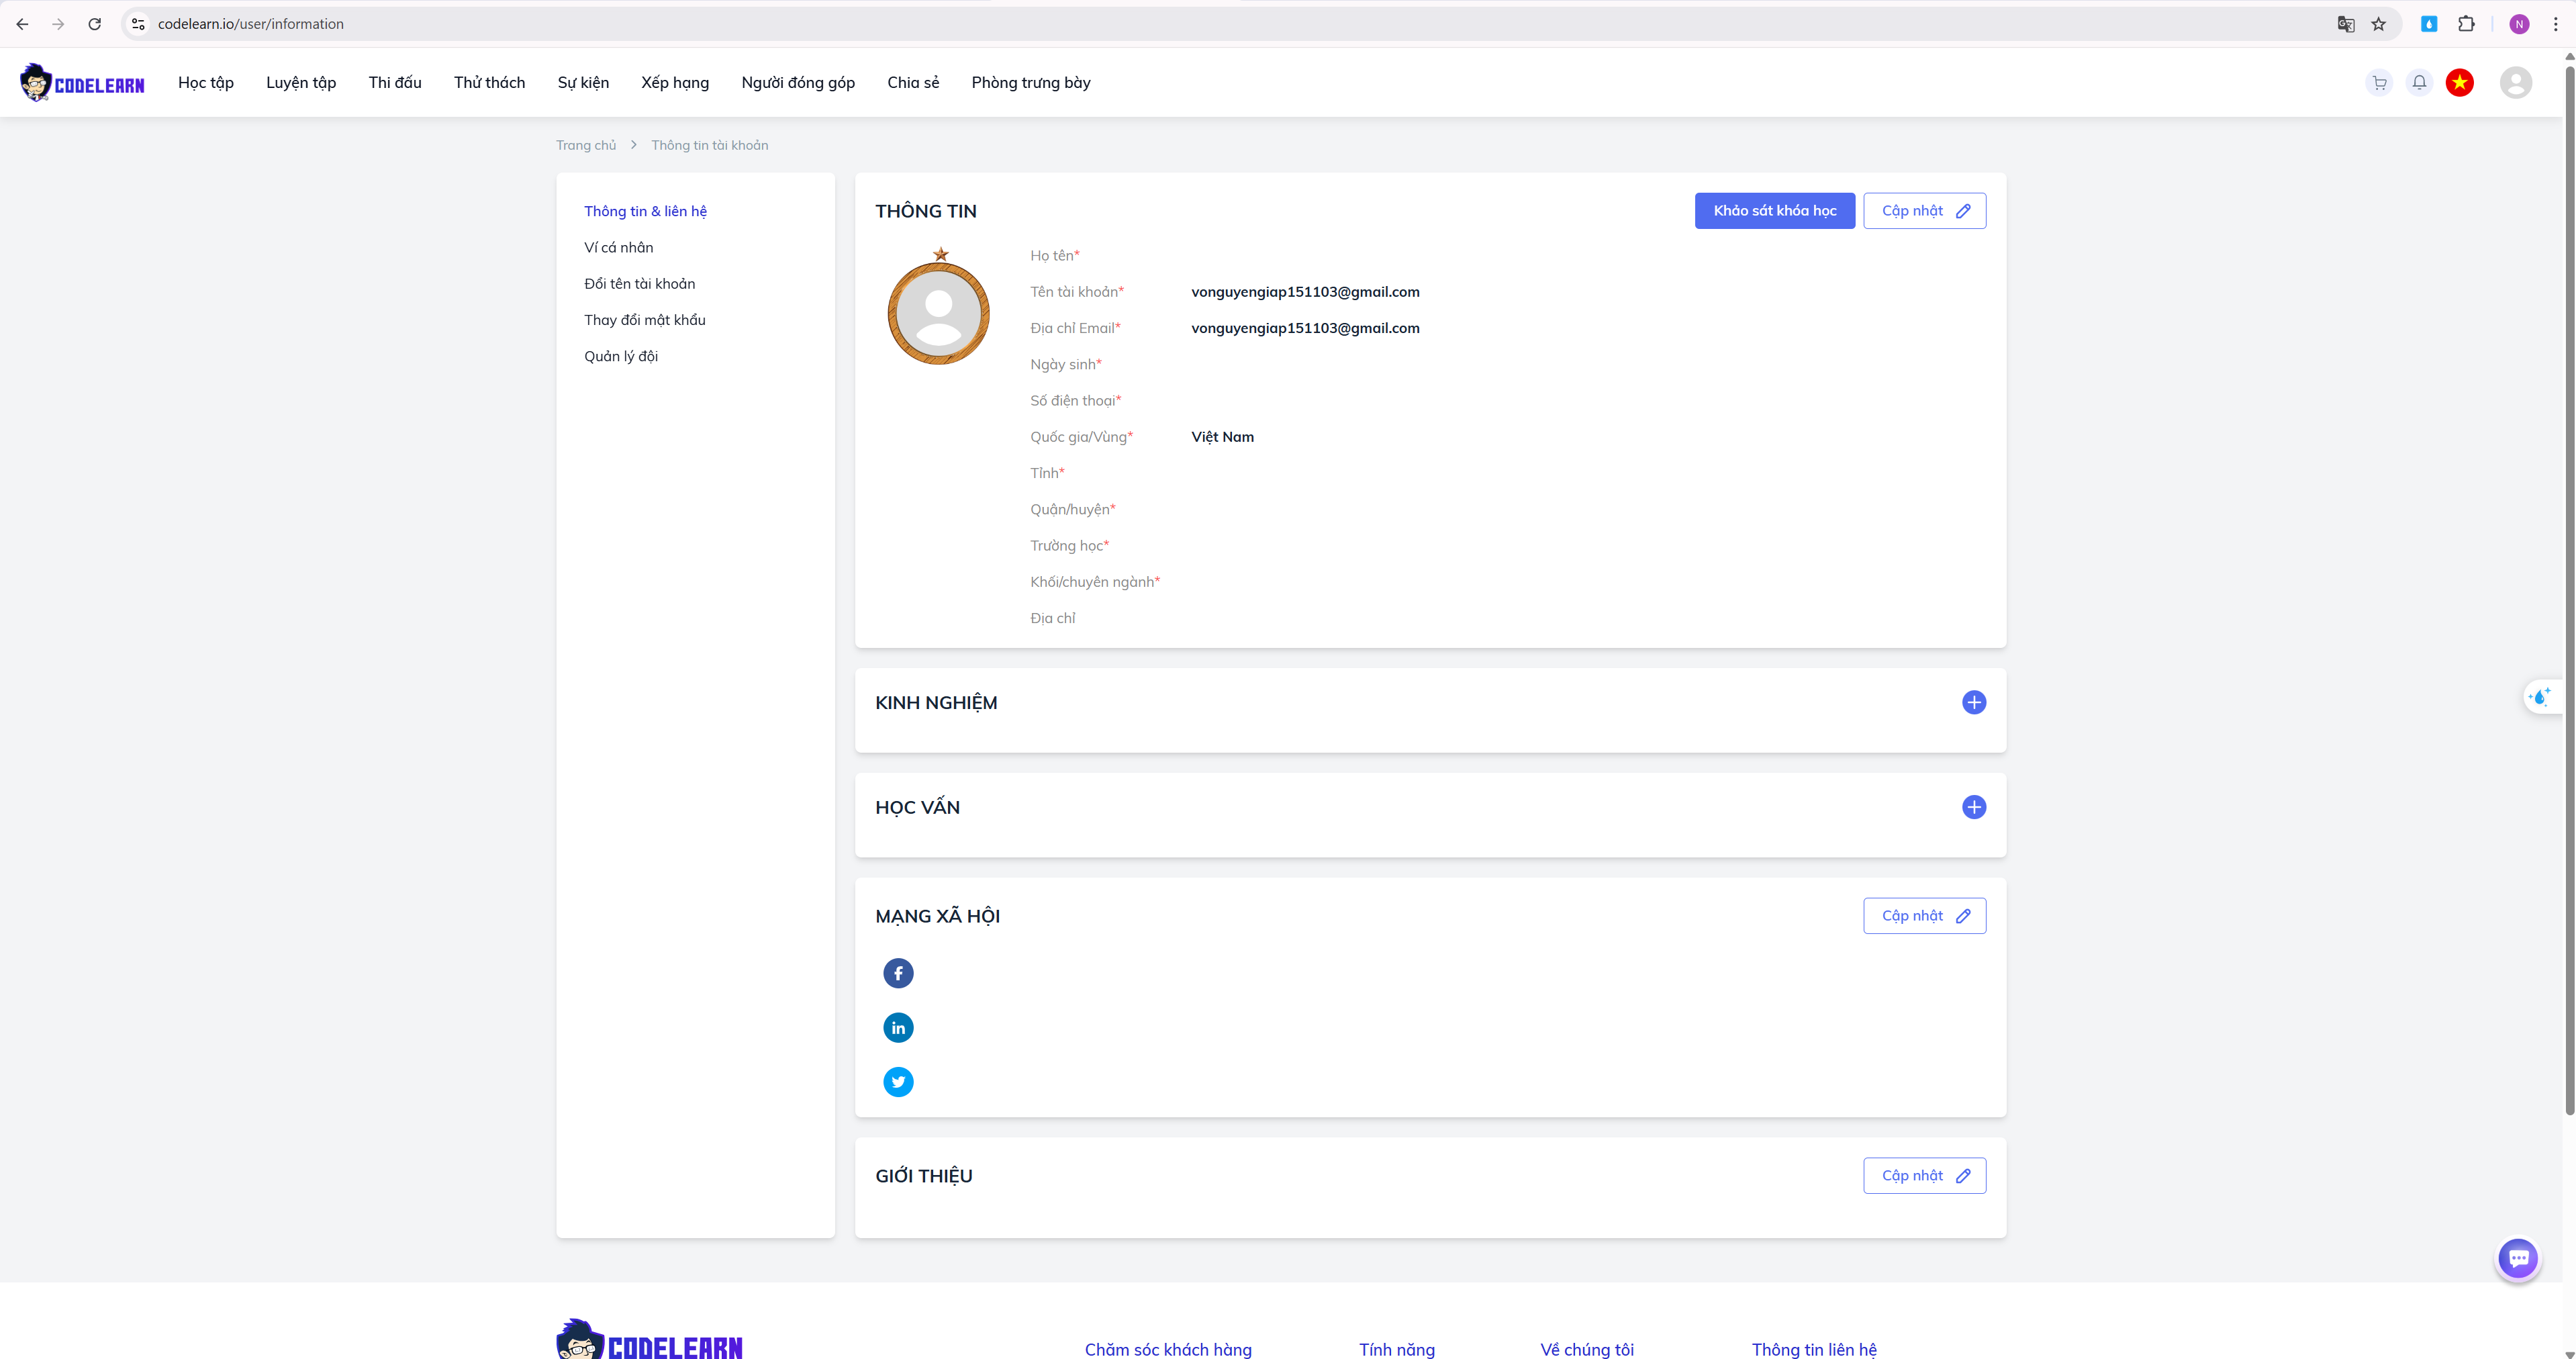
\includegraphics[width=1\linewidth]{picture/minh_chung_1.png}
    \caption{Thông tin của người đăng ký}
\end{figure}

\begin{figure}[!htp]
    \centering
    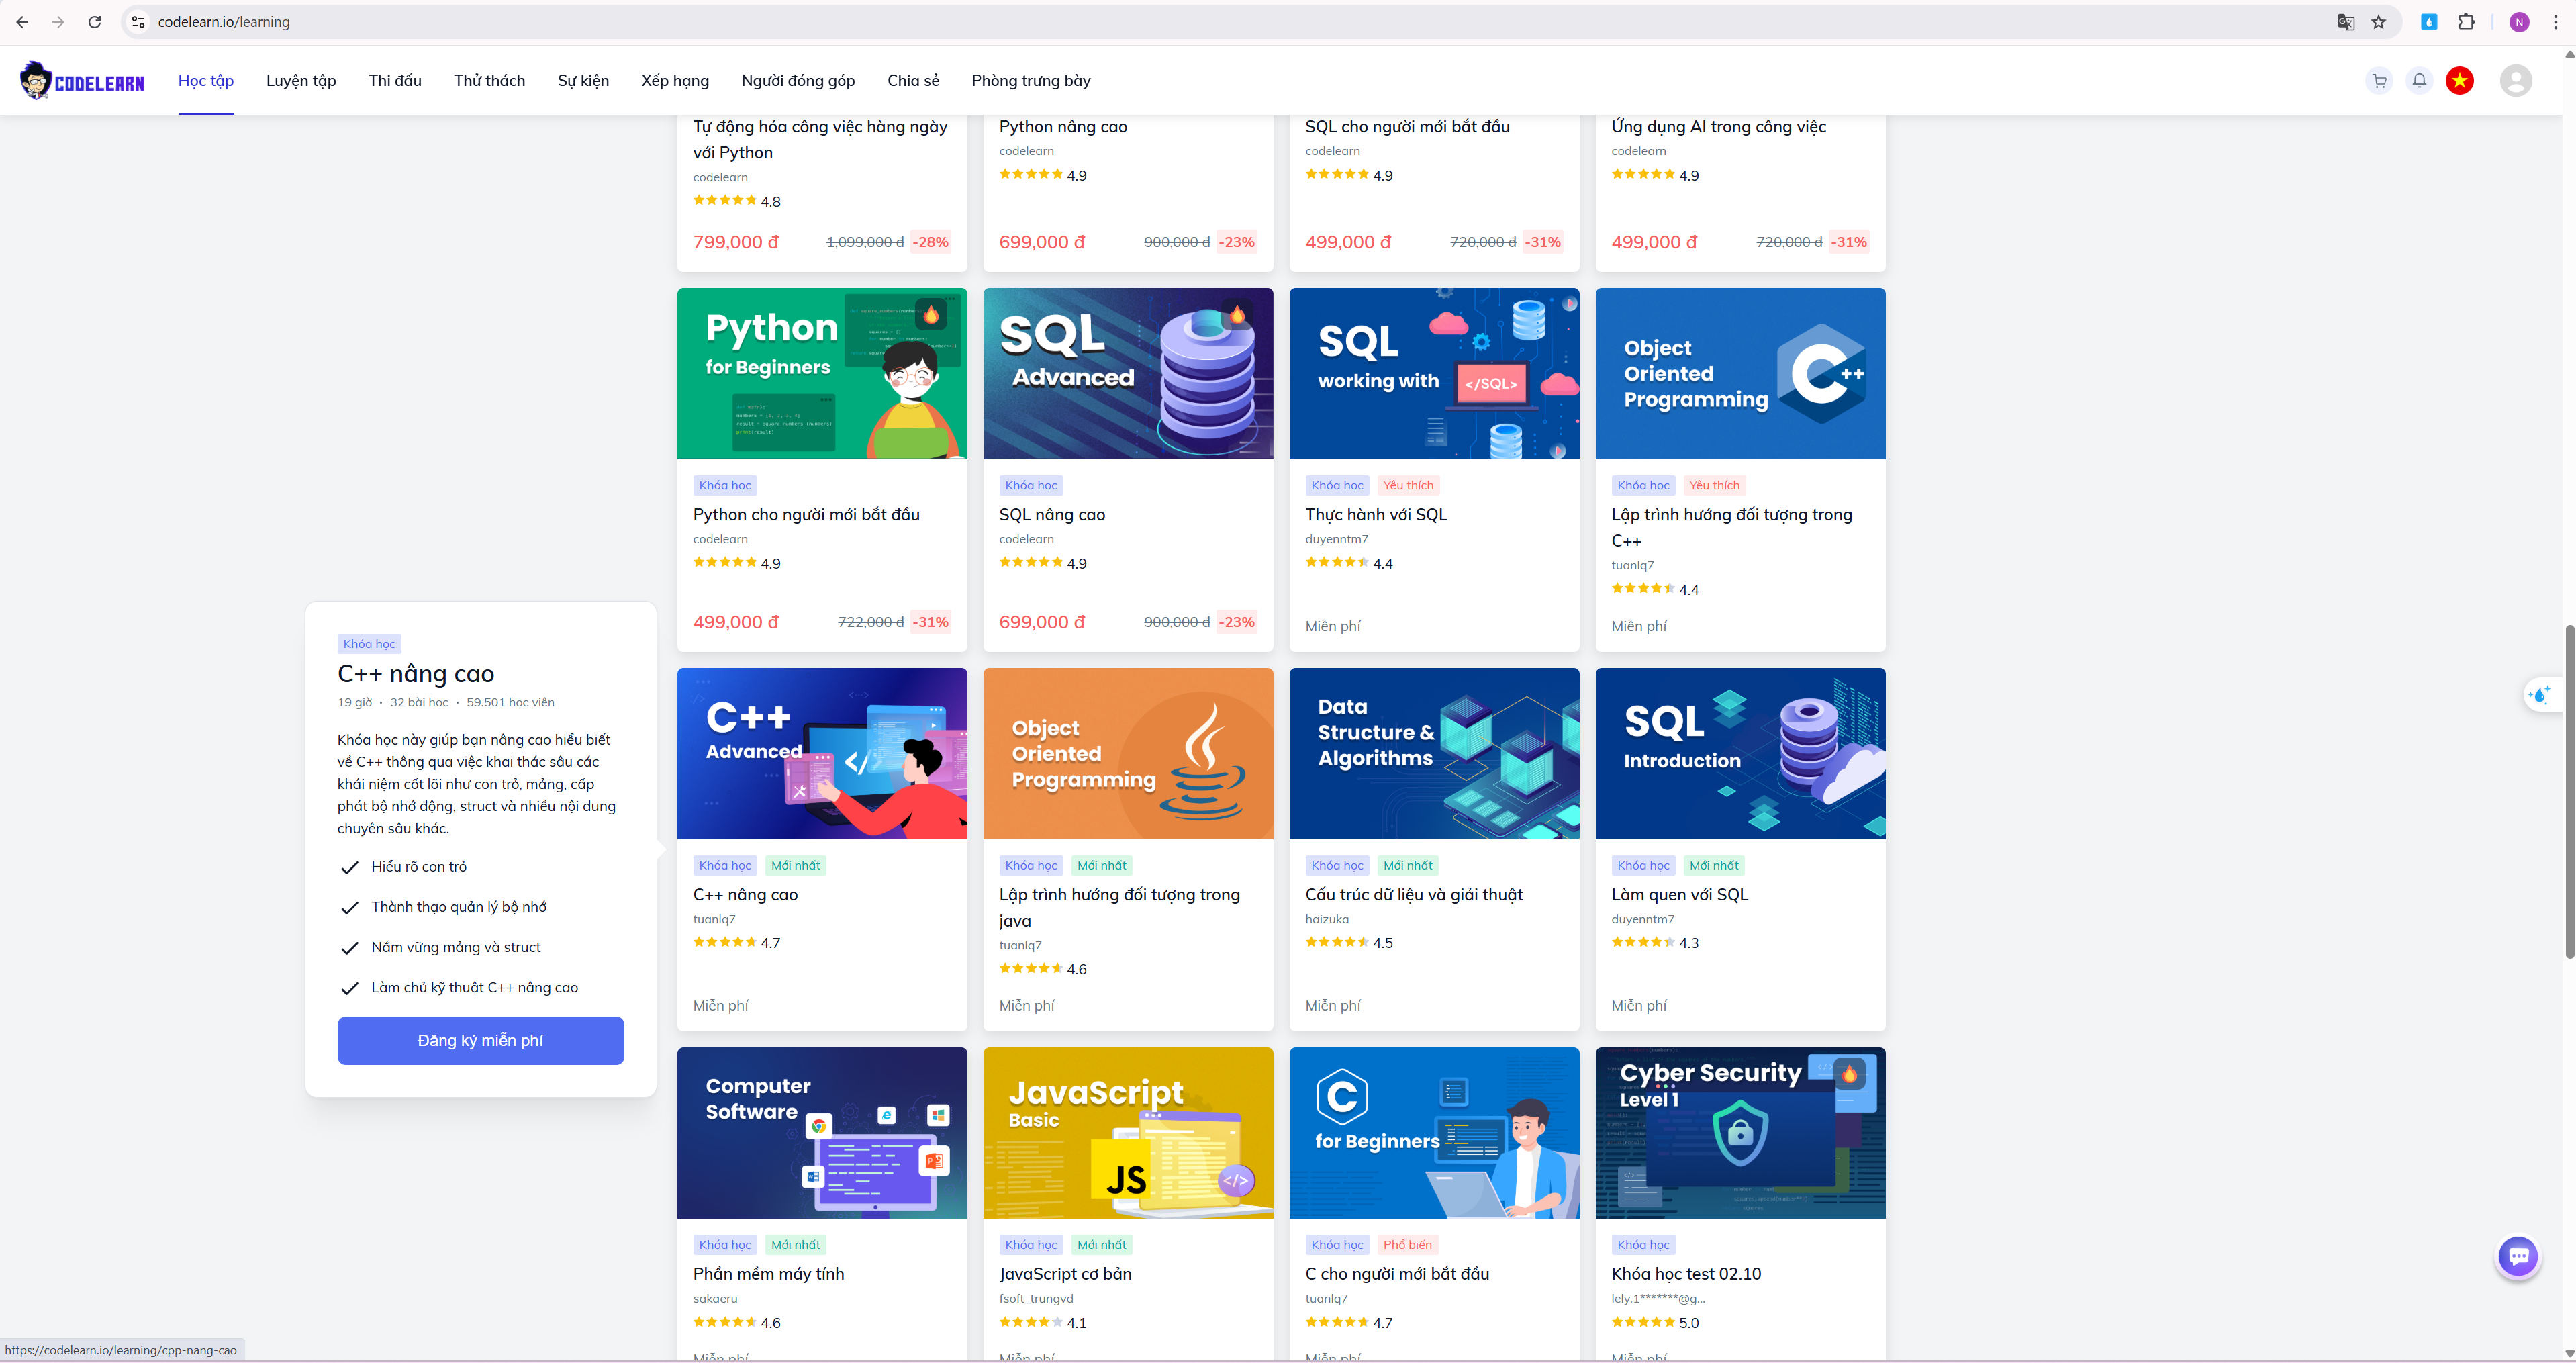
\includegraphics[width=1\linewidth]{picture/minh_chung_2.png}
    \caption{Thông tin về các khóa học}
\end{figure}

\begin{figure}[!htp]
    \centering
    
\includegraphics[width=1\linewidth]{picture/minh_chung_3.png}
    \caption{Thông tin chi tiết một khoá học}
\end{figure}

\begin{figure}[!htp]
    \centering
    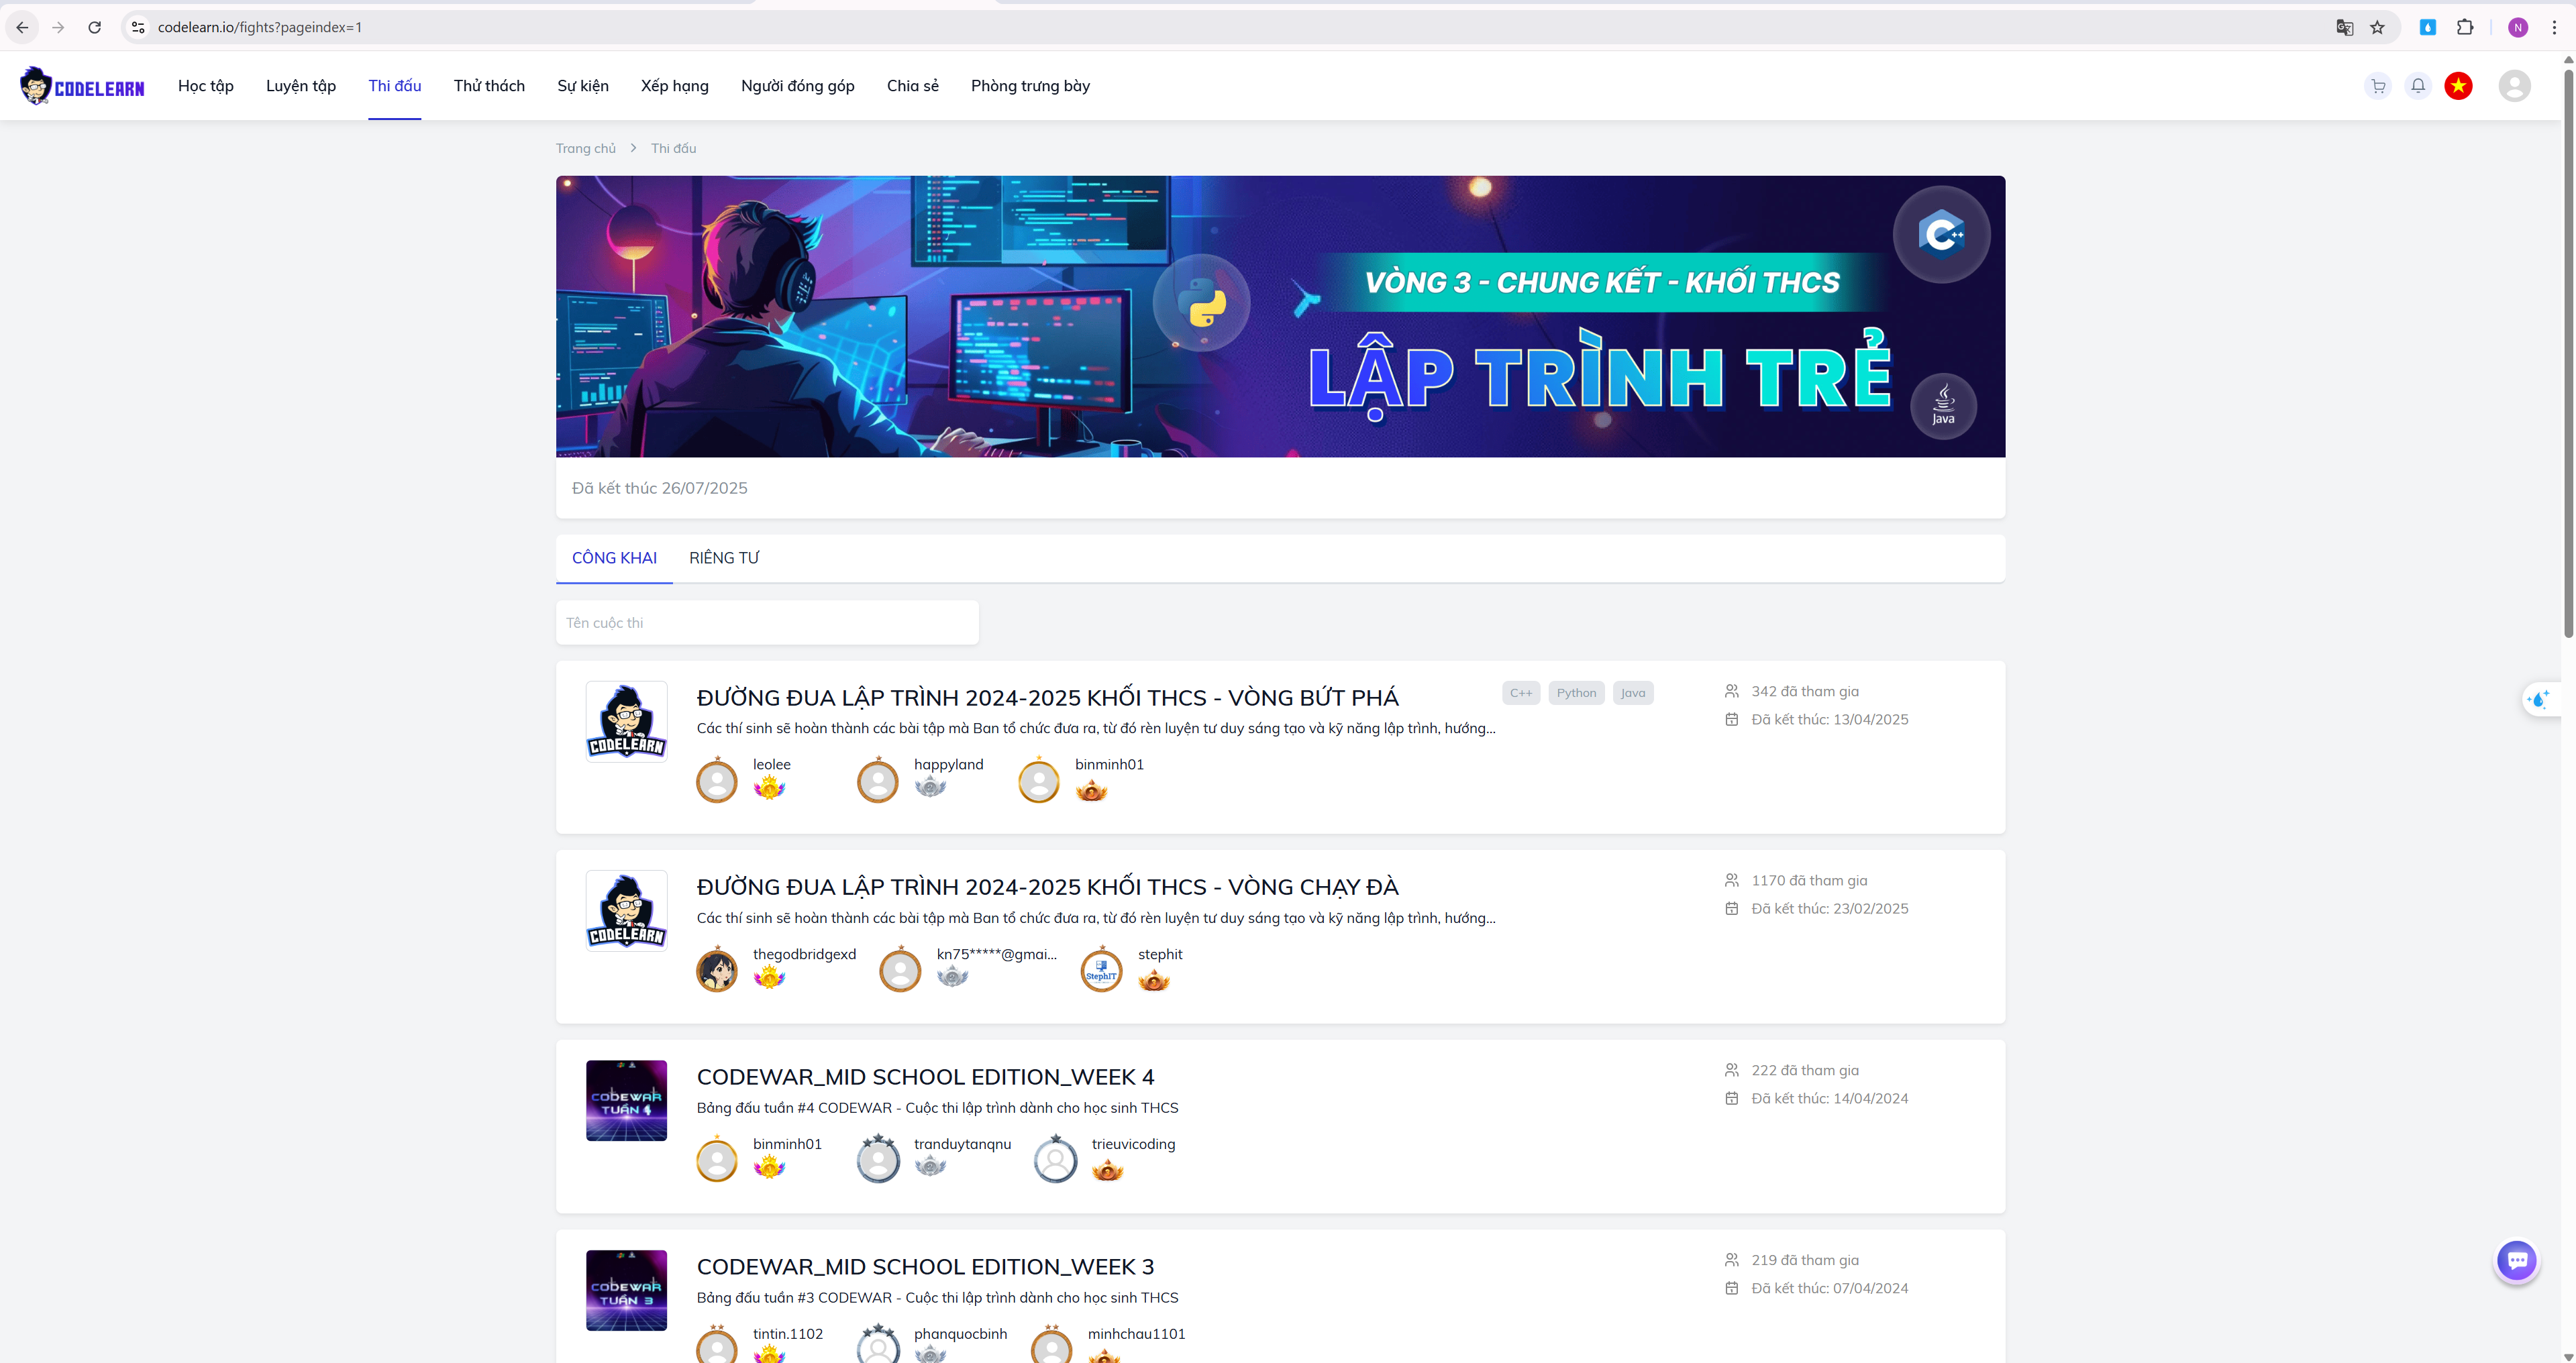
\includegraphics[width=1\linewidth]{picture/minh_chung_4.png}
    \caption{Thông tin về các cuộc thi}
\end{figure}

\begin{figure}
    \centering
    
\includegraphics[width=1\linewidth]{picture/minh_chung_6.png}
    \caption{Thông tin về các bài chia sẻ}
\end{figure}

\begin{figure}[!htp]
    \centering
    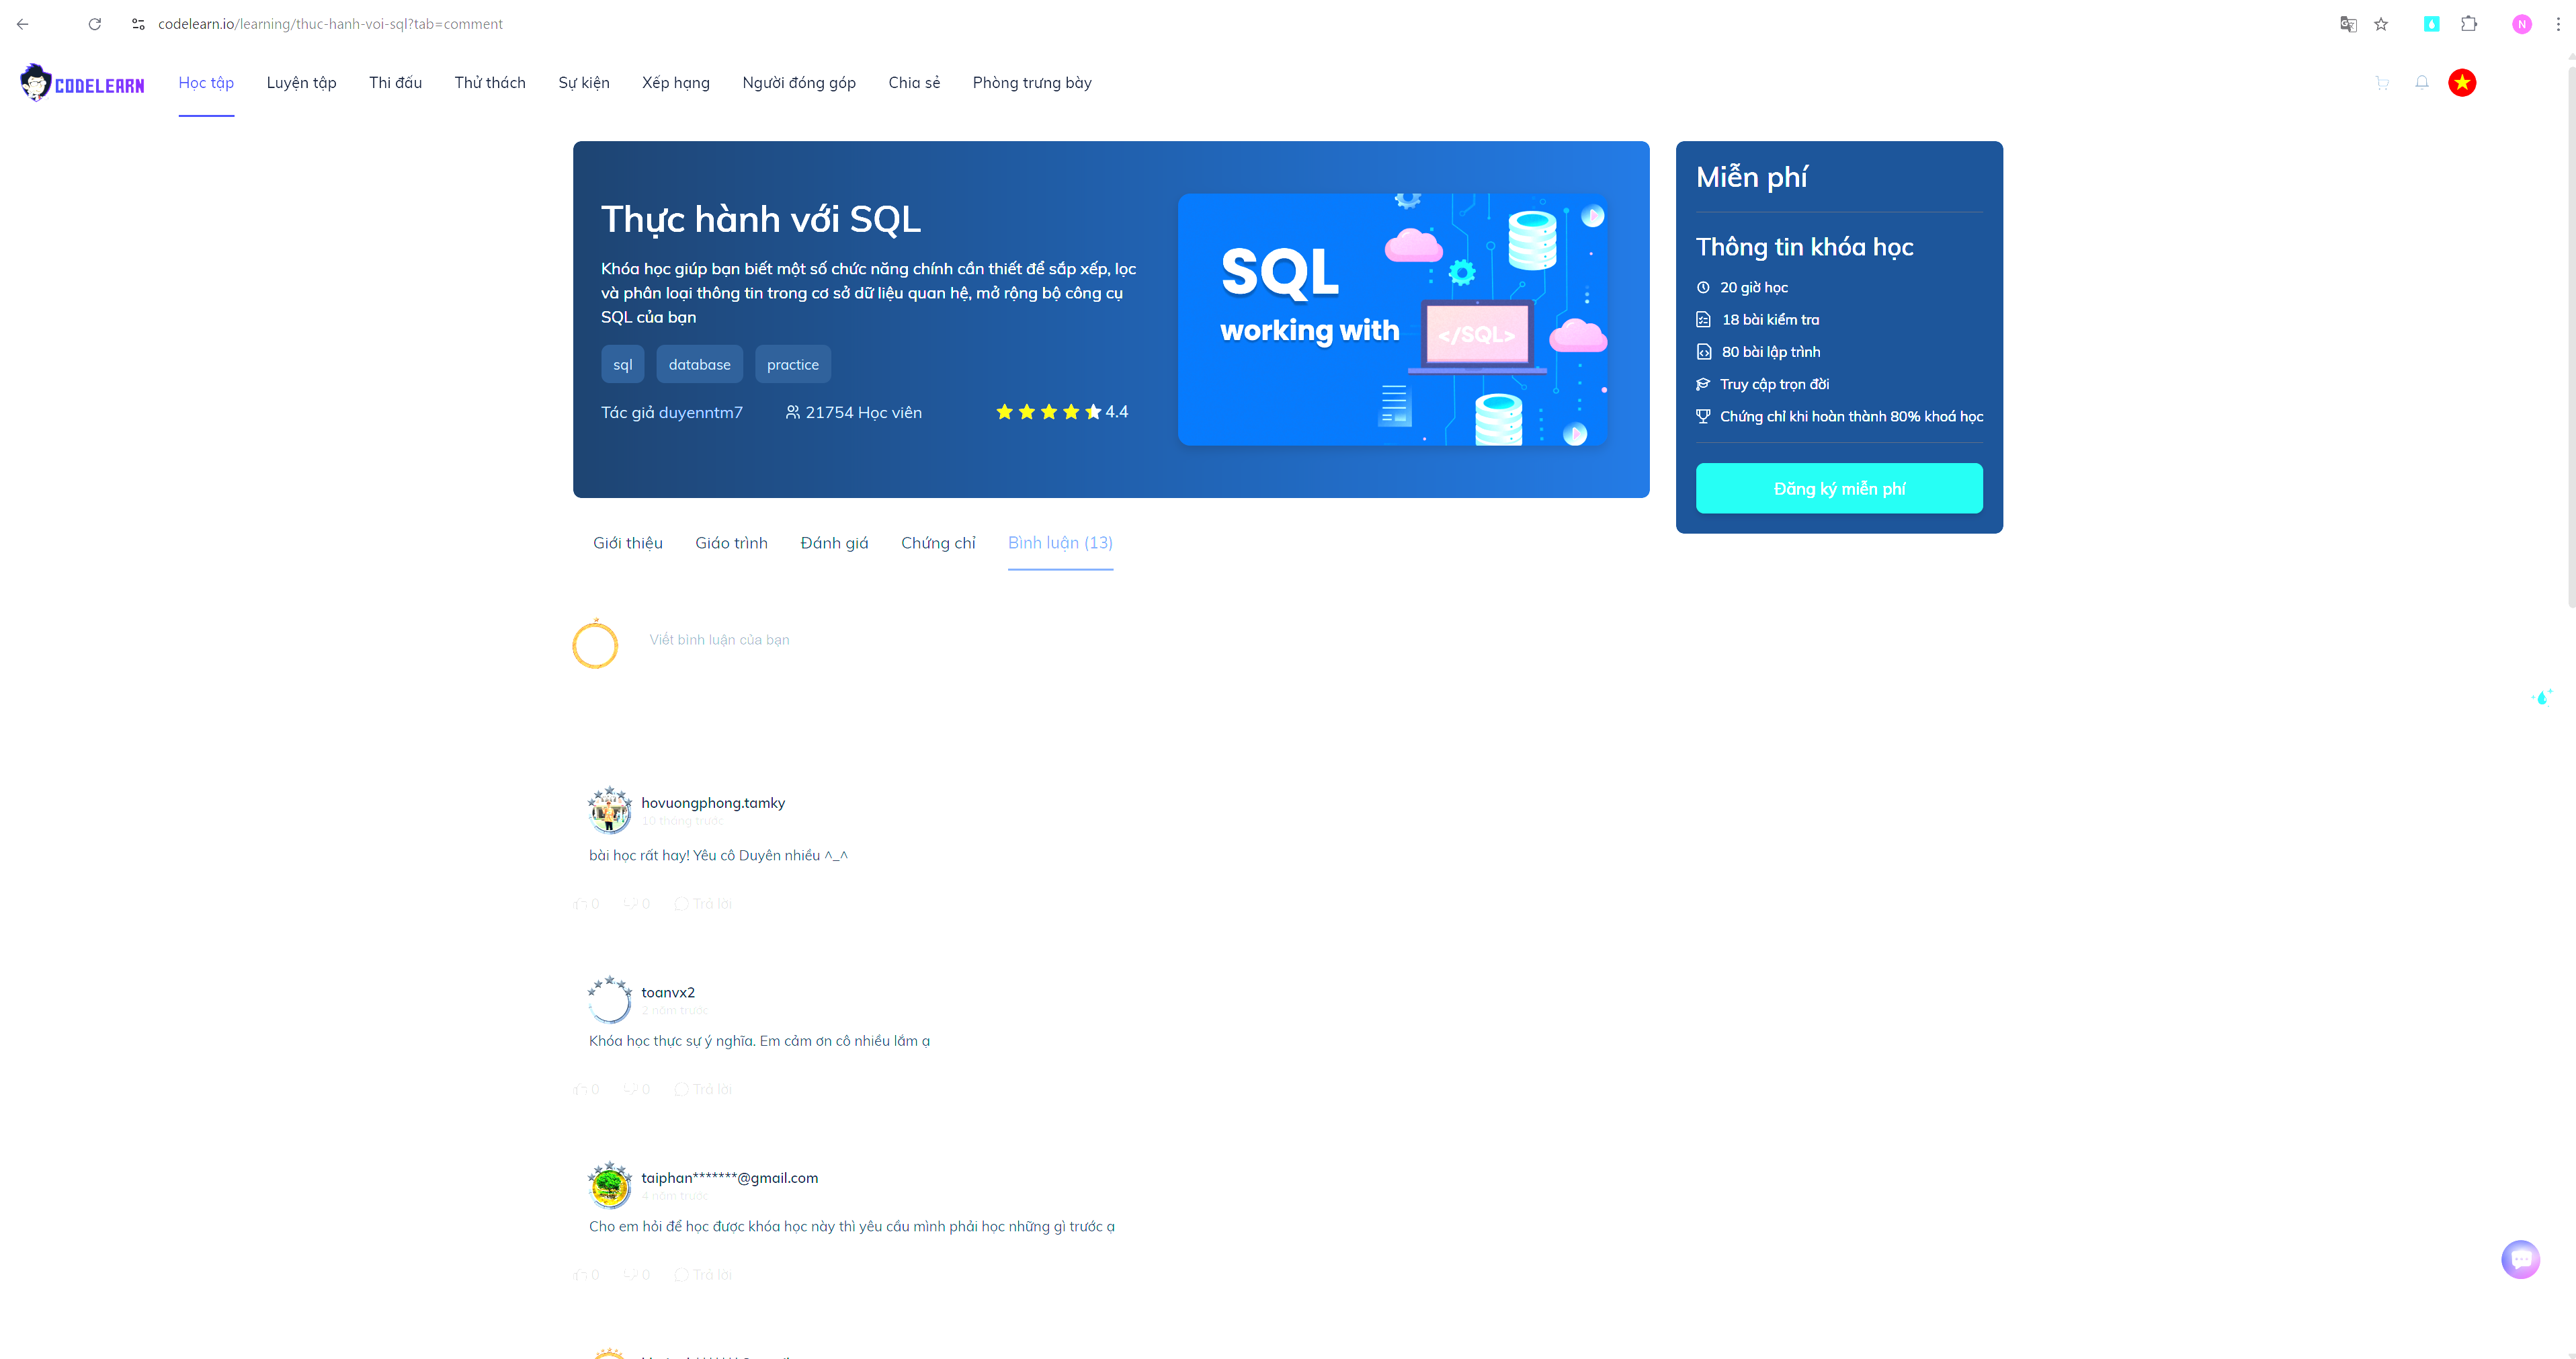
\includegraphics[width=1\linewidth]{picture/minh_chung_5.png}
    \caption{Thông tin về bình luận, đánh giá}
\end{figure}
\subsection{Mô tả hệ thống đề xuất}
\subsubsection{Mô tả tổng quan}
Hệ thống E-Learning được thiết kế để quản lý toàn diện hoạt động dạy và học trực tuyến, đáp ứng nhu cầu ngày càng cao về đào tạo từ xa. Hệ thống tập trung vào việc xây dựng một môi trường học tập linh hoạt, có cấu trúc rõ ràng và tương tác cao giữa các thành phần tham gia.

Mỗi khóa học trong hệ thống được xây dựng và quản lý bởi một giáo viên phụ trách. Giáo viên có toàn quyền thiết kế nội dung giảng dạy thông qua việc tổ chức khóa học thành các chương học khác nhau. Trong mỗi chương, giáo viên có thể bố trí nhiều bài học với đa dạng hình thức, bao gồm bài học lý thuyết thông thường và video bài giảng, cùng với hệ thống bài tập và bài kiểm tra đi kèm để đánh giá năng lực người học.

Người học khi tham gia hệ thống có thể đăng ký vào nhiều khóa học khác nhau. Trong mỗi khóa học, họ sẽ được trải nghiệm lộ trình học tập được sắp xếp khoa học theo từng chương, thực hiện các bài tập để củng cố kiến thức và tham gia các bài kiểm tra để đánh giá mức độ tiếp thu. Bên cạnh đó, hệ thống còn cung cấp các bài luyện tập độc lập không thuộc chương trình cụ thể nào, cho phép người học rèn luyện thêm kỹ năng.

Để tăng cường tính tương tác, hệ thống tích hợp diễn đàn thảo luận thông qua các bài viết chia sẻ và bình luận. Mỗi bài viết đều được đăng bởi một người dùng cụ thể và có thể thu hút nhiều bình luận từ cộng đồng. Đặc biệt, hệ thống bình luận được thiết kế theo dạng đa cấp, cho phép người dùng phản hồi trực tiếp đến các bình luận khác, tạo nên những chuỗi thảo luận sôi nổi và mang tính xây dựng cao.

Hệ thống cũng chú trọng đến việc đánh giá chất lượng khóa học thông qua cơ chế cho điểm và nhận xét từ người học. Mỗi khóa học sẽ hiển thị điểm đánh giá trung bình dựa trên các đánh giá từ những người đã tham gia, giúp người học mới có cái nhìn tổng quan về chất lượng khóa học trước khi đăng ký.

Với kiến trúc module rõ ràng và khả năng mở rộng cao, hệ thống E-Learning hướng đến việc trở thành một nền tảng học tập trực tuyến toàn diện, đáp ứng mọi nhu cầu về đào tạo từ cơ bản đến nâng cao cho cả cá nhân và tổ chức.

\subsubsection{Mô tả các kiểu thực thể, các thuộc tính, mối liên kết}
Mỗi \textbf{NGƯỜI DÙNG} sẽ có một \textit{\underline{mã số tài khoản}} để định danh. Các thông tin cá nhân cần lưu trữ bao gồm \underline{\textit{tên tài khoản}}, \textit{mật khẩu}, \textit{email}, \textit{số điện thoại}, \textit{họ tên}, \textit{địa chỉ}, địa chỉ được chi tiết hóa thành \textit{phường, tỉnh, quốc gia}. Hệ thống cũng ghi nhận \textit{ngày tham gia} và quản lý \textit{trạng thái tài khoản} như hoạt động hoặc bị khóa. Người dùng có thể \textbf{tham gia} vào nhiều khóa học, đồng thời \textbf{đánh giá} các khóa học mà họ đã học. Họ cũng có thể \textbf{thực hiện} các bài luyện tập, bài tập và bài kiểm tra trong hệ thống. Ngoài ra, người dùng còn có thể \textbf{đăng} các bài viết chia sẻ và \textbf{viết} bình luận để tương tác với cộng đồng.

\textbf{GIÁO VIÊN} cũng là người dùng, được cung cấp vai trò để \textbf{tạo} các khóa học và các bài luyện tập. Giáo viên kế thừa tất cả thuộc tính từ người dùng thông thường và có thêm các thông tin về học vấn như \textit{trường đào tạo}, \textit{chuyên ngành}, cùng \textit{thời gian bắt đầu} và \textit{thời gian kết thúc} tham gia giảng dạy. Mỗi giáo viên có thể tạo và quản lý nhiều khóa học, bài luyện tập khác nhau.

Mỗi \textbf{KHÓA HỌC} trong hệ thống được xác định duy nhất bằng \underline{\textit{mã số khóa học}}. Thông tin về khóa học bao gồm \underline{\textit{tên khóa học}} và \textit{trạng thái hiện tại} như đang mở hoặc đóng. Để cung cấp cái nhìn tổng quan cho người học, khóa học còn lưu trữ các số liệu thống kê quan trọng như \textit{số lượng bài tập}, \textit{số lượng bài kiểm tra}, \textit{số lượng bài lý thuyết}, \textit{số lượng video}, \textit{tổng thời lượng}, \textit{số lượng học viên đã tham gia}, \textit{số lượt đánh giá} và \textit{điểm đánh giá trung bình} từ những người đã học.

Mỗi khóa học được tạo ra bởi một giáo viên duy nhất và có thể thu hút nhiều người dùng tham gia. Người dùng tham gia khóa học không chỉ học tập mà còn có thể đánh giá chất lượng khóa học đó. Cấu trúc nội dung của khóa học được tổ chức thông qua các chương học, mỗi khóa học có thể bao gồm nhiều chương khác nhau.

Mỗi \textbf{CHƯƠNG} được xác định bằng \underline{\textit{mã số chương}} và có \textit{tên chương} trong khóa học để phản ánh nội dung chính của chương đó.

Mỗi chương luôn \textbf{thuộc về} một khóa học cụ thể. Trong mỗi chương có thể chứa nhiều \textit{bài học} khác nhau, tạo thành lộ trình học tập tuần tự cho người học. Ngoài ra, chương còn có thể \textbf{bao gồm} các bài tập và bài kiểm tra nhằm đánh giá mức độ tiếp thu kiến thức của người học sau khi hoàn thành chương học. Bài học trong hệ thống được phân thành hai dạng chính: \textit{bài học lý thuyết} và \textit{video bài học}. Với bài học lý thuyết, nội dung trong bài học sẽ được giáo viên soạn trực tiếp và lưu trong hệ thống. Còn với video bài học, giáo viên sẽ dẫn \textit{URL của video} được lưu trên nền tảng khác để giảm tải việc lưu dữ liệu.

\textbf{BÀI TẬP} được thiết kế để giúp người học củng cố kiến thức đã học trong từng chương. Mỗi bài tập có \underline{\textit{mã số bài tập}} và các thông tin mô tả bao gồm \textit{tên bài tập}, \textit{nội dung đề bài}, \textit{đáp án mẫu} để người học tham khảo và \textit{điểm đạt} tối thiểu cần đạt được.

Mỗi bài tập luôn thuộc về một chương cụ thể, giúp người học có thể luyện tập và áp dụng những kiến thức vừa học trong chương đó. Việc này đảm bảo tính liên kết chặt chẽ giữa nội dung học và phần thực hành.

\textbf{BÀI KIỂM TRA} đóng vai trò đánh giá năng lực và mức độ tiếp thu của người học sau khi hoàn thành mỗi chương học. Mỗi bài kiểm tra có \underline{\textit{mã số bài kiểm tra}}, cùng với tên bài \textit{kiểm tra}, \textit{thời gian làm bài} quy định, \textit{điểm đạt} chuẩn và \textit{tổng điểm} của toàn bài.

Bài kiểm tra luôn gắn liền với một chương học cụ thể. Nhiều người dùng có thể thực hiện cùng một bài kiểm tra, và hệ thống sẽ ghi nhận đầy đủ thông tin cho mỗi lần thực hiện bao gồm \textit{thời gian nộp bài}, \textit{điểm số đạt được} và \textit{số thứ tự} lần nộp bài. Mỗi bài kiểm tra \textbf{có bao gồm} một số lượng câu hỏi nhất định, trả lời các câu hỏi để số điểm làm bài kiểm tra đạt mức được thông qua.

Mỗi \textbf{CÂU HỎI} được xác định bằng \textit{số thứ tự }trong bài kiểm tra và có \textit{nội dung} câu hỏi cụ thể cùng với \textit{số điểm} tương ứng cho câu hỏi đó.

Mỗi câu hỏi luôn thuộc về một bài kiểm tra duy nhất. Đi cùng với mỗi câu hỏi là nhiều \textit{câu trả lời} khác nhau để người học lựa chọn. Câu trả lời là các phương án lựa chọn cho mỗi câu hỏi. Mỗi câu trả lời chứa nội dung cụ thể và có thể được đánh dấu là đáp án đúng hoặc sai, giúp hệ thống có thể tự động chấm điểm cho bài kiểm tra. Một câu hỏi có thể có một hoặc nhiều đáp án đúng tùy theo giáo viên ra đề.

\textbf{BÀI LUYỆN TẬP} là dạng bài tập đặc biệt, không gắn trực tiếp với bất kỳ chương học cụ thể nào, cho phép người học thực hành kiến thức một cách linh hoạt và không giới hạn điều kiện. Mỗi bài luyện tập có \underline{\textit{mã số bài luyện tập}}, cùng với \underline{\textit{tên bài luyện tập}}, \textit{đề bài} và thông tin về \textit{độ khó}. Độ khó của mỗi bài luyện tập được chia ra làm dễ, trung bình hoặc khó.

Nhiều người dùng có thể thực hiện cùng một bài luyện tập, và mỗi người dùng cũng có thể thực hiện nhiều bài luyện tập khác nhau. Hệ thống sẽ ghi nhận chi tiết \textit{thời gian làm bài}, \textit{thời điểm nộp bài} và \textit{điểm số} đạt được cho mỗi lần thực hiện, giúp người học theo dõi được sự tiến bộ của mình.

\textbf{BÀI VIẾT CHIA SẺ} tạo nên diễn đàn thảo luận chung trong hệ thống, nơi người dùng có thể chia sẻ kiến thức, kinh nghiệm học tập. Mỗi bài viết có \underline{\textit{mã số bài viết}}, cùng với \underline{\textit{tên bài viết}}, \textit{nội dung chi tiết} và \textit{ngày đăng bài}.

Mỗi bài viết luôn được đăng bởi một người dùng cụ thể, và người dùng đó chịu trách nhiệm về nội dung mà mình chia sẻ với cộng đồng.

\textbf{BÌNH LUẬN} là công cụ tương tác quan trọng trong hệ thống, cho phép người dùng trao đổi ý kiến ở nhiều ngữ cảnh khác nhau. Mỗi bình luận có \underline{\textit{mã số bình luận riêng biệt}}, cùng với \textit{nội dung bình luận} và \textit{thời gian đăng}.

Mỗi bình luận đều được viết bởi một người dùng cụ thể. Bình luận có thể \textbf{được gắn với} các bài viết chia sẻ hoặc khóa học, tạo thành những cuộc thảo luận sôi nổi. Đặc biệt, hệ thống hỗ trợ tính năng bình luận đa cấp, trong đó một bình luận có thể \textbf{có bao gồm} một bình luận phản hồi khác, tạo thành cấu trúc hội thoại dạng cây. Những bình luận gốc sẽ được theo dõi thông qua \textit{số lượt trả lời}, phản ánh mức độ tương tác của cộng đồng với chủ đề đó.

\subsubsection{Mô tả các ràng buộc ngữ nghĩa về các kiểu thực thể, thuộc tính, mối liên kết mà không biểu diễn được bằng (E-)ERD}
Dù thành công trong mô hình hóa cấu trúc dữ liệu hệ thống thông tin, song mô hình ERD vẫn có giới hạn. Một số ràng buộc ngữ nghĩa thực tế không thể biểu diễn thông qua ERD, có thể kể đến như: \vspace{-0.3cm}
\begin{enumerate}
\item Người dùng bị khóa tài khoản (bị cấm) không thể đăng bài viết, bình luận hoặc tham gia bất kỳ hoạt động học tập nào. \vspace{-0.3cm}
\item Khóa học chỉ được mở cho người học đăng ký khi trạng thái là “hoạt động” (active). \vspace{-0.3cm}
\item Giáo viên không thể đăng ký tham gia khóa học do chính mình tạo ra. \vspace{-0.3cm}
\item Chỉ tác giả của khóa học mới được quyền chỉnh sửa nội dung trong khóa học. \vspace{-0.3cm}
\item Một người dùng chỉ có thể thực hiện bài tập trong các khóa học mà họ đã đăng ký. \vspace{-0.3cm}
\item Một người dùng chỉ có thể thực hiện bài kiểm tra trong các khóa học mà họ đã đăng ký. \vspace{-0.3cm}
\item Điểm đánh giá của người dùng phải nằm trong khoảng 1–5 sao. \vspace{-0.3cm}
\item Người dùng chỉ có thể đánh giá khóa học đã đăng ký. \vspace{-0.3cm}
\item Người dùng chỉ được đánh giá mỗi khóa học một lần. \vspace{-0.3cm}
\item Người học chỉ có thể nộp bài tối đa 10 lần/ngày cho cùng một bài luyện tập. \vspace{-0.3cm}
\item Điểm số bài luyện tập không thể âm và tối đa là 100 điểm. \vspace{-0.3cm}
\item Một người dùng chỉ có thể đăng tối đa 5 bài viết trong 1 ngày. \vspace{-0.3cm}
\end{enumerate}
\section{Thiết kế EERD}
\begin{figure}[H]
    \centering
    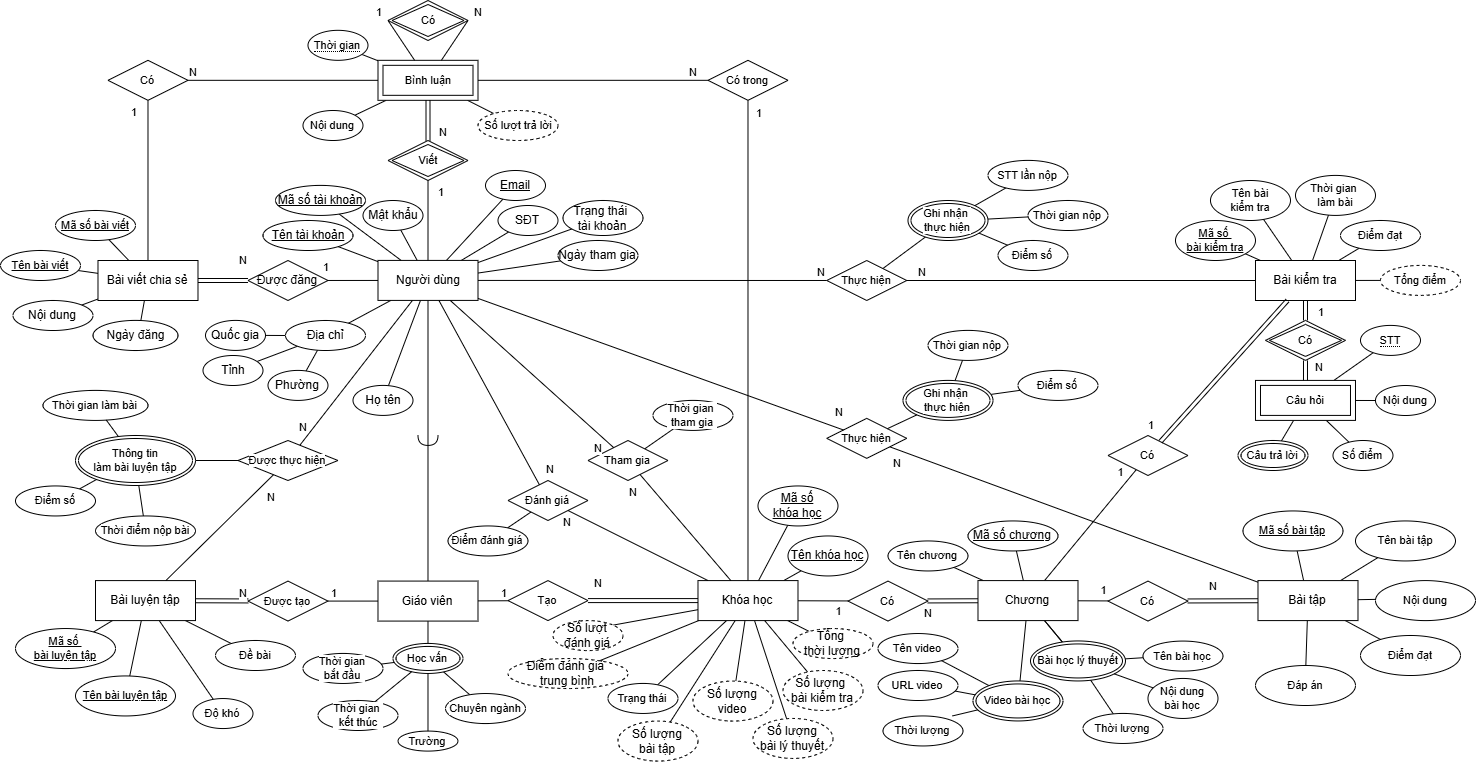
\includegraphics[width=1\linewidth]{picture/ERD.drawio.png}
    \caption{EERD trang web học trực tuyến}
    \label{fig:placeholder}
\end{figure}
Toàn bộ mô hình EERD chi tiết được lưu tại liên kết sau:
\href{https://app.diagrams.net/#G1XY2dIsVTmTCCmIWk3s_vGwzFGodUWAKx#%7B%22pageId%22%3A%22BJtFvQvSTNEqXKE1NMD3%22%7D}{\textbf{Xem EERD chi tiết tại đây}}.
\newpage
\begin{figure}[H]
    \centering
    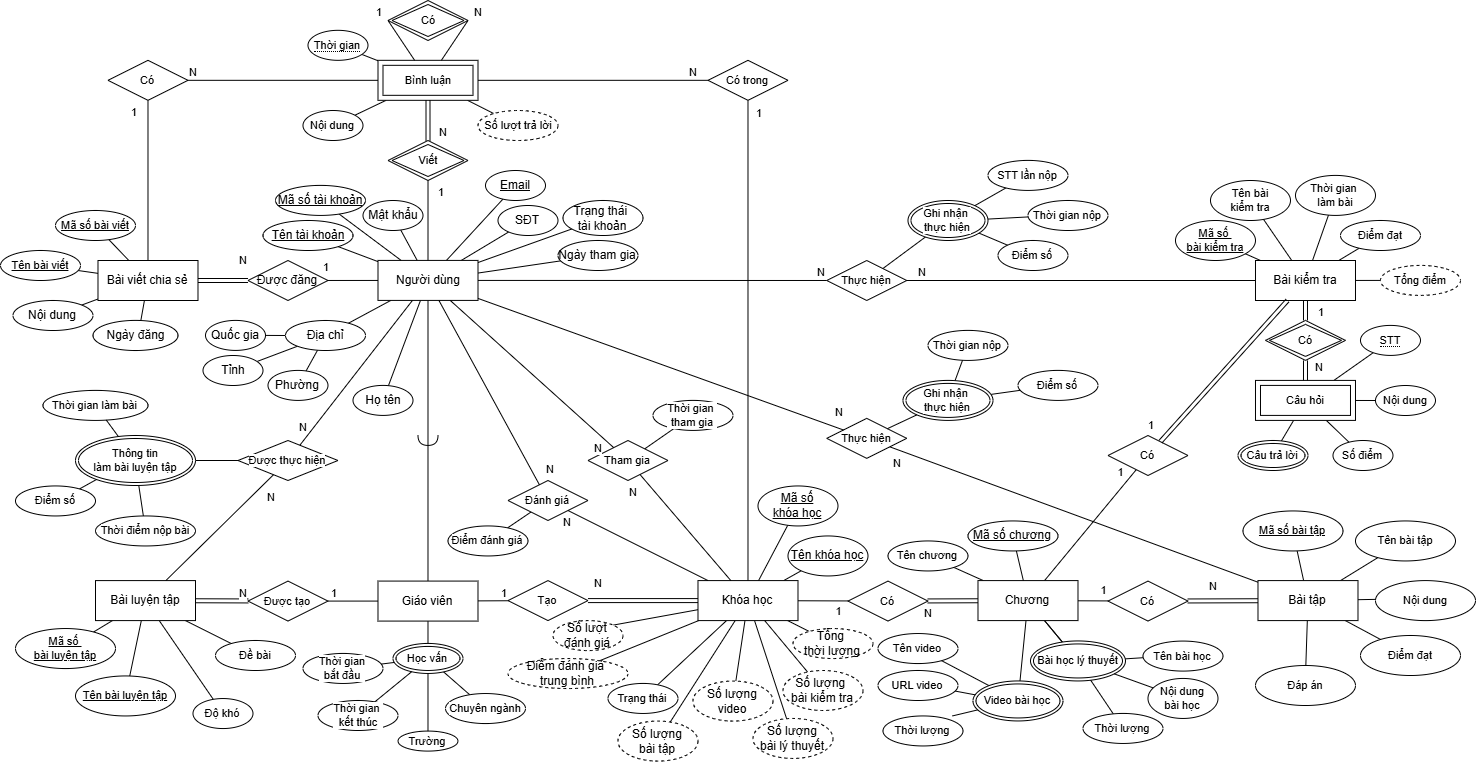
\includegraphics[angle=-90, width=0.7\linewidth]{picture/ERD.drawio.png}
    \caption{EERD trang web học trực tuyến (ảnh nằm ngang)}
    \label{fig:placeholder}
\end{figure}
\section{Ánh xạ sang lược đồ CSDL}
Dựa trên phương pháp ánh xạ đã được học, nhóm sinh viên ánh xạ qua lược đồ cơ sở dữ liệu theo thứ tự sau:

\subsection{Bước 1: Ánh xạ các kiểu thực thể mạnh (Regular Entity Types)}
Thực thể mạnh bao gồm: \textbf{NGƯỜI DÙNG}, \textbf{KHÓA HỌC}, \textbf{CHƯƠNG}, \textbf{BÀI TẬP}, \textbf{BÀI KIỂM TRA}, \textbf{BÀI LUYỆN TẬP} và \textbf{BÀI VIẾT CHIA SẺ}. Tất nhiên các quan hệ dưới đây sẽ có thêm khóa ngoại khi chúng tham gia vào các mối liên kết mà sẽ được hoàn thiện ở các bước sau.
\begin{figure}[H]
    \centering
    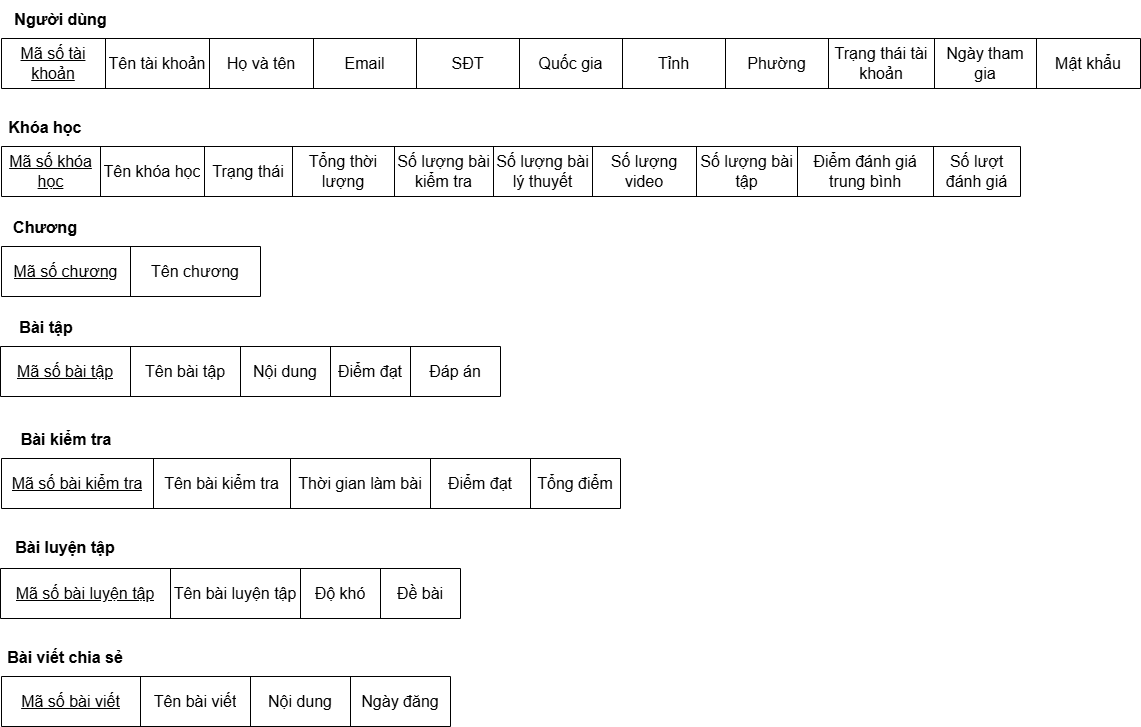
\includegraphics[width=1\linewidth]{picture/TTmanh.png}
    \caption{Bước 1: Ánh xạ các kiểu thực thể mạnh (Regular Entity Types)}
    \label{fig:placeholder}
\end{figure}
\subsection{Bước 2: Ánh xạ các kiểu thực thể yếu (Weak Entity Types)}
\textbf{BÌNH LUẬN} là thực thể yếu, khóa của thực thể này bao gồm cả khóa ngoại (Mã số tài khoản) và khóa riêng phần của chính nó (Thời gian).

\textbf{CÂU HỎI} là thực thể yếu, khóa của thực thể này bao gồm cả khóa ngoại (Mã số bài kiểm tra) và khóa riêng phần (STT).
\begin{figure}[H]
    \centering
    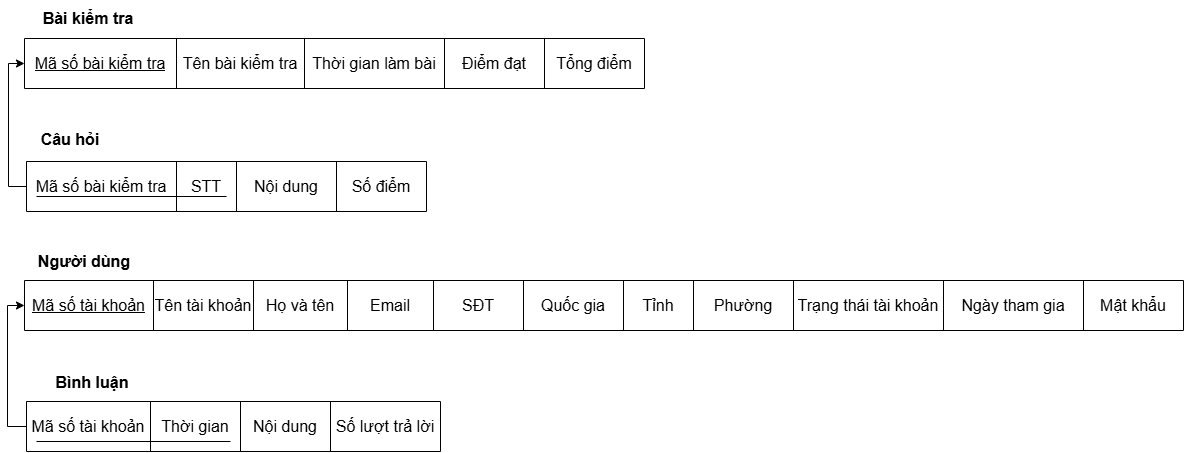
\includegraphics[width=1\linewidth]{picture/TTyeu.png}
    \caption{Bước 2: Ánh xạ các kiểu thực thể yếu (Weak Entity Types)}
    \label{fig:placeholder}
\end{figure}
\vspace{-20pt}
\subsection{Bước 3: Ánh xạ các kiểu mối liên kết hai ngôi 1:1 (Binary	1:1	Relationship Types)}
Mỗi \textbf{CHƯƠNG} có một \textbf{BÀI KIỂM TRA}, nên ta đưa khóa chính của \textbf{CHƯƠNG} vào làm  khóa ngoại của \textbf{BÀI KIỂM TRA} để thể hiện mối liên kết \textbf{có} 1:1. \vspace{-12pt}
\begin{figure}[H]
    \centering
    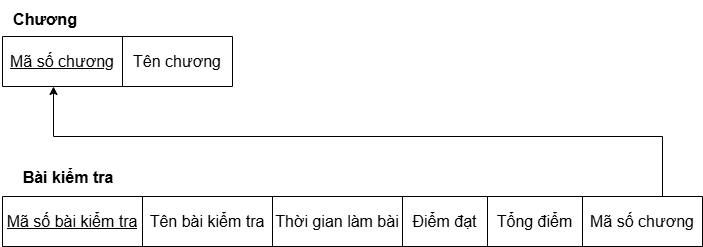
\includegraphics[width=0.75\linewidth]{picture/lk1-1.png}
    \caption{Bước 3: Ánh xạ các kiểu mối liên kết hai ngôi 1:1 (Binary	1:1	Relationship Types)}
    \label{fig:placeholder}
\end{figure}
\subsection{Bước 4: Ánh xạ các kiểu mối liên kết hai ngôi 1:N (Binary	1:N	Relationship Types)}
\textbf{NGƯỜI DÙNG} \textbf{đăng} \textbf{BÀI VIẾT},

\textbf{NGƯỜI DÙNG} \textbf{viết} \textbf{BÌNH LUẬN},

\textbf{GIÁO VIÊN} \textbf{tạo} \textbf{KHÓA HỌC},

\textbf{GIÁO VIÊN} \textbf{tạo} \textbf{BÀI LUYỆN TẬP},

\textbf{KHÓA HỌC} \textbf{có} \textbf{CHƯƠNG}, 

\textbf{KHÓA HỌC} \textbf{có} \textbf{BÌNH LUẬN},

\textbf{CHƯƠNG} \textbf{có} \textbf{BÀI TẬP},

\textbf{BÀI KIỂM TRA} \textbf{có} \textbf{CÂU HỎI},

\textbf{BÀI VIẾT CHIA SẺ} \textbf{có} \textbf{BÌNH LUẬN},

\textbf{BÌNH LUẬN} \textbf{có} \textbf{BÌNH LUẬN} khác phản hồi là các mối liên kết hai ngôi 1:N.
\begin{figure}[H]
    \centering
    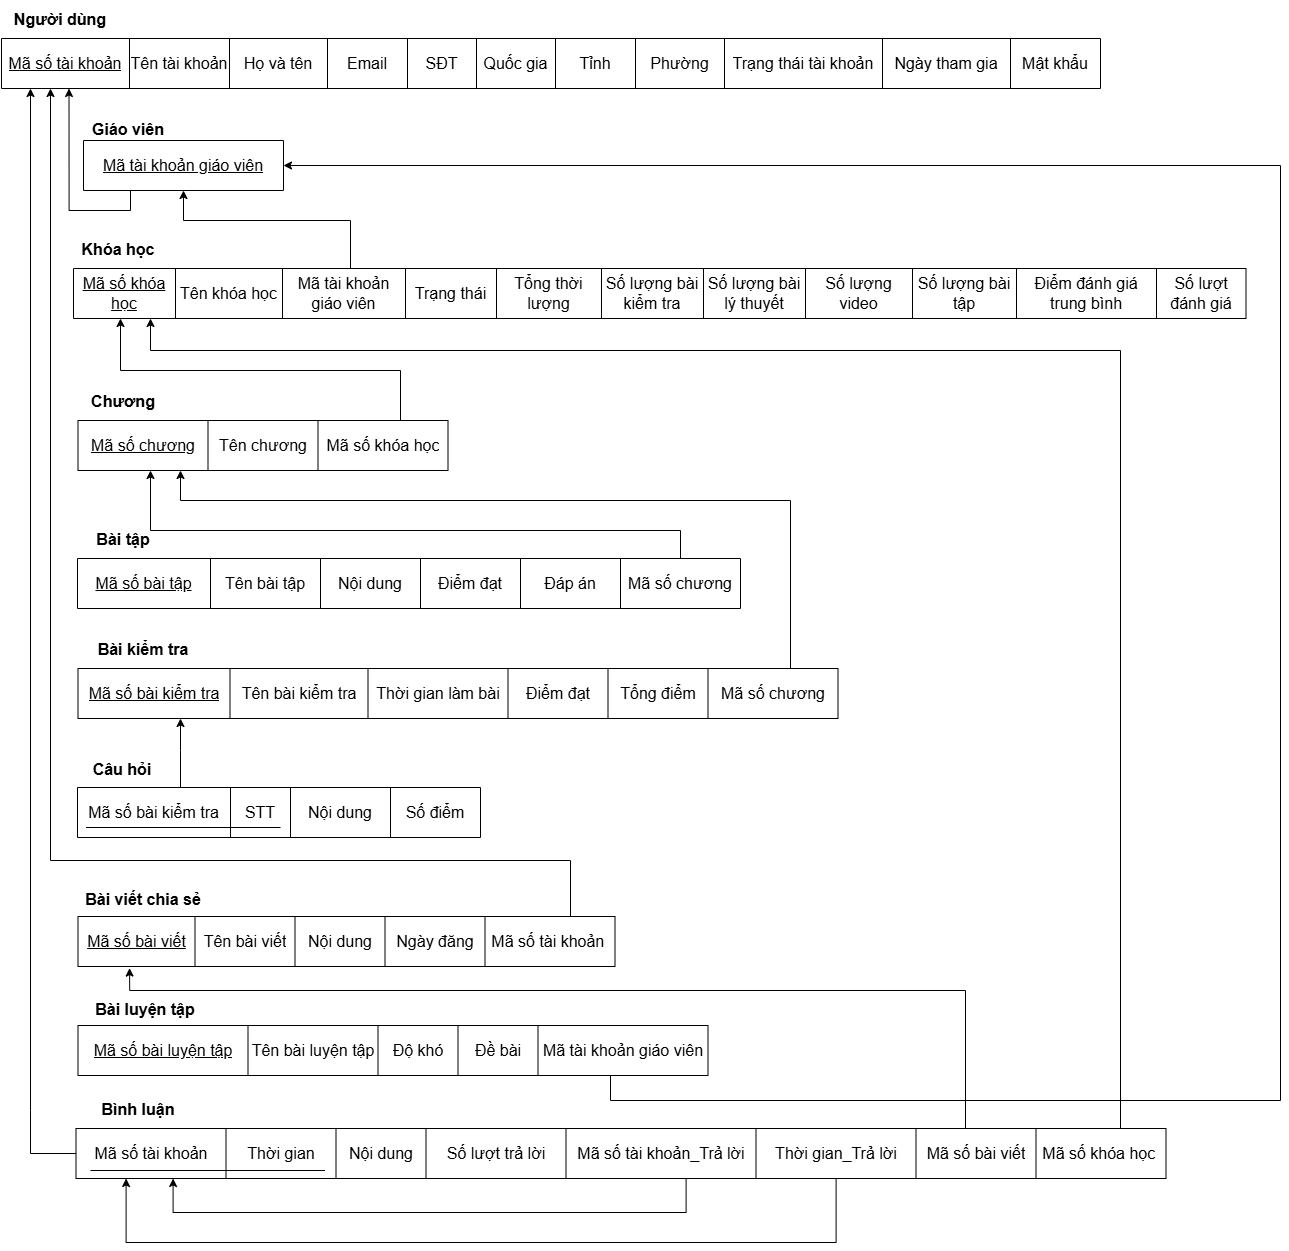
\includegraphics[width=1\linewidth]{picture/lk1-n.png}
    \caption{Bước 4: Ánh xạ các kiểu mối liên kết hai ngôi 1:N (Binary	1:N	Relationship Types)}
    \label{fig:placeholder}
\end{figure}
\vspace{-30pt}
\subsection{Bước 5: Ánh xạ các kiểu mối liên kết hai ngôi N:N (Binary	N:N	Relationship Types)}
\textbf{NGƯỜI DÙNG} \textbf{thực hiện} \textbf{BÀI KIỂM TRA}, 

\textbf{NGƯỜI DÙNG} \textbf{thực hiện} \textbf{BÀI TẬP},

\textbf{NGƯỜI DÙNG} \textbf{thực hiện} \textbf{BÀI LUYỆN TẬP},

\textbf{NGƯỜI DÙNG} \textbf{tham gia} \textbf{KHÓA HỌC},

\textbf{NGƯỜI DÙNG} \textbf{đánh giá} \textbf{KHÓA HỌC} là các mối liên kết hai ngôi N:N.
\begin{figure}[H]
    \centering
    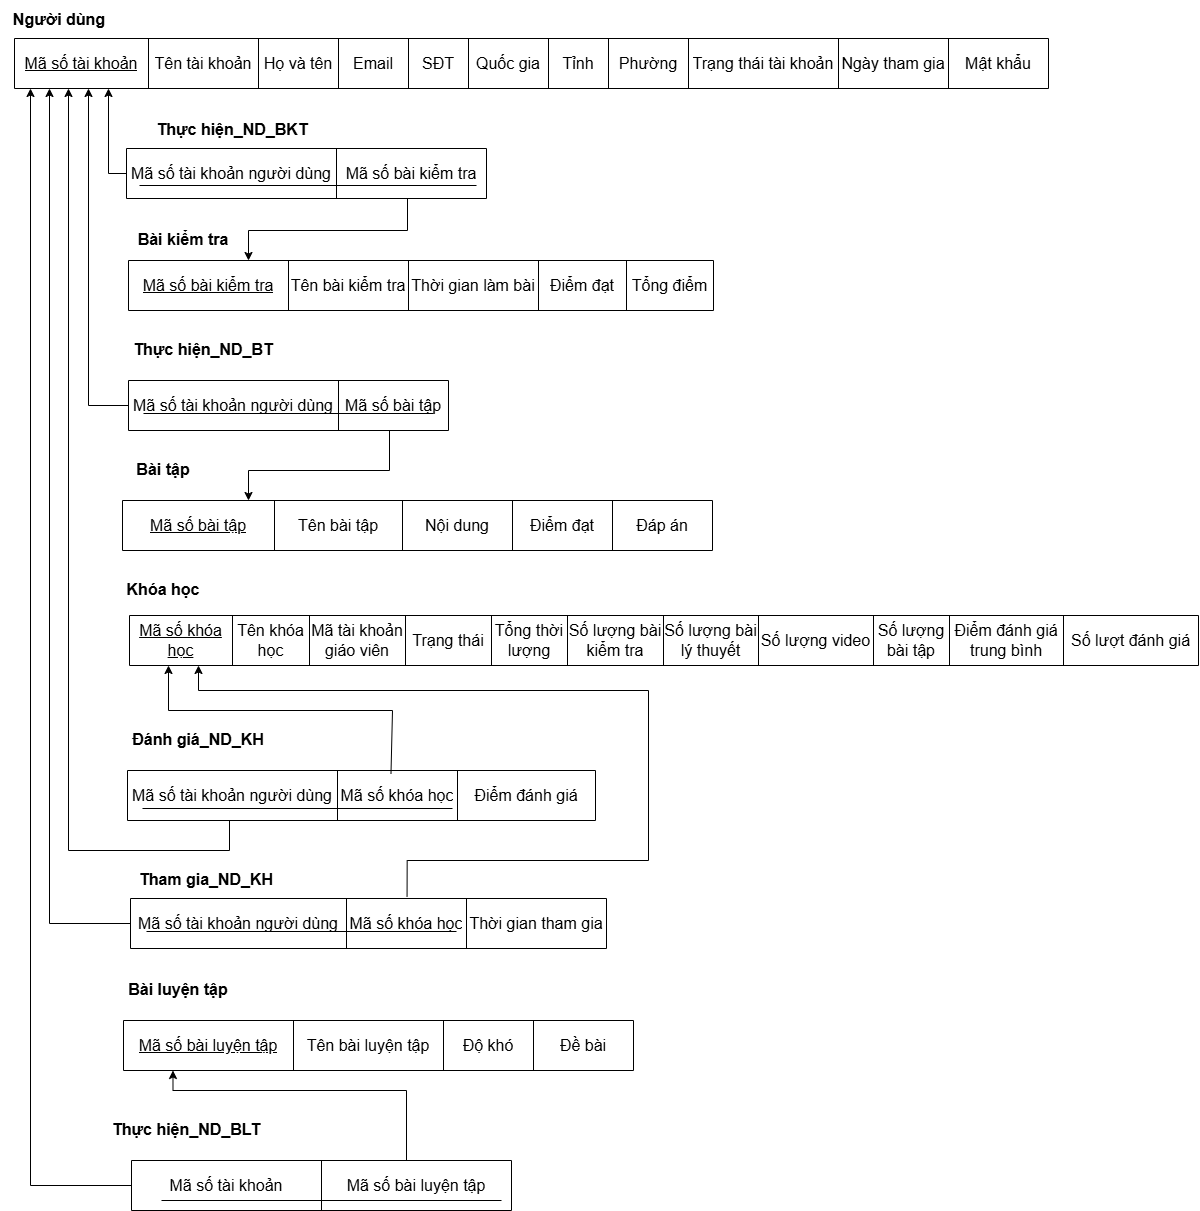
\includegraphics[width=1\linewidth]{picture/lkn-n.png}
    \caption{Bước 5: Ánh xạ các kiểu mối liên kết hai ngôi N:N (Binary	N:N	Relationship Types)}
    \label{fig:placeholder}
\end{figure}
\vspace{-40pt}
\subsection{Bước 6: Ánh xạ các thuộc tính đa trị (Multivalued	attributes)} \vspace{-4pt}
Các thuộc tính đa trị gồm: Video bài học, Bài học lý thuyết của \textbf{CHƯƠNG}, Ghi nhận thực hiện của mối liên kết \textbf{NGƯỜI DÙNG thực hiện BÀI TẬP}, Ghi nhận thực hiện của mối liên kết \textbf{NGƯỜI DÙNG thực hiện BÀI KIỂM TRA}, Học vấn của \textbf{GIÁO VIÊN}, Thông tin làm bài luyện tập của mối liên kết \textbf{NGƯỜI DÙNG thực hiện BÀI LUYỆN TẬP}.
\begin{figure}[H]
    \centering
    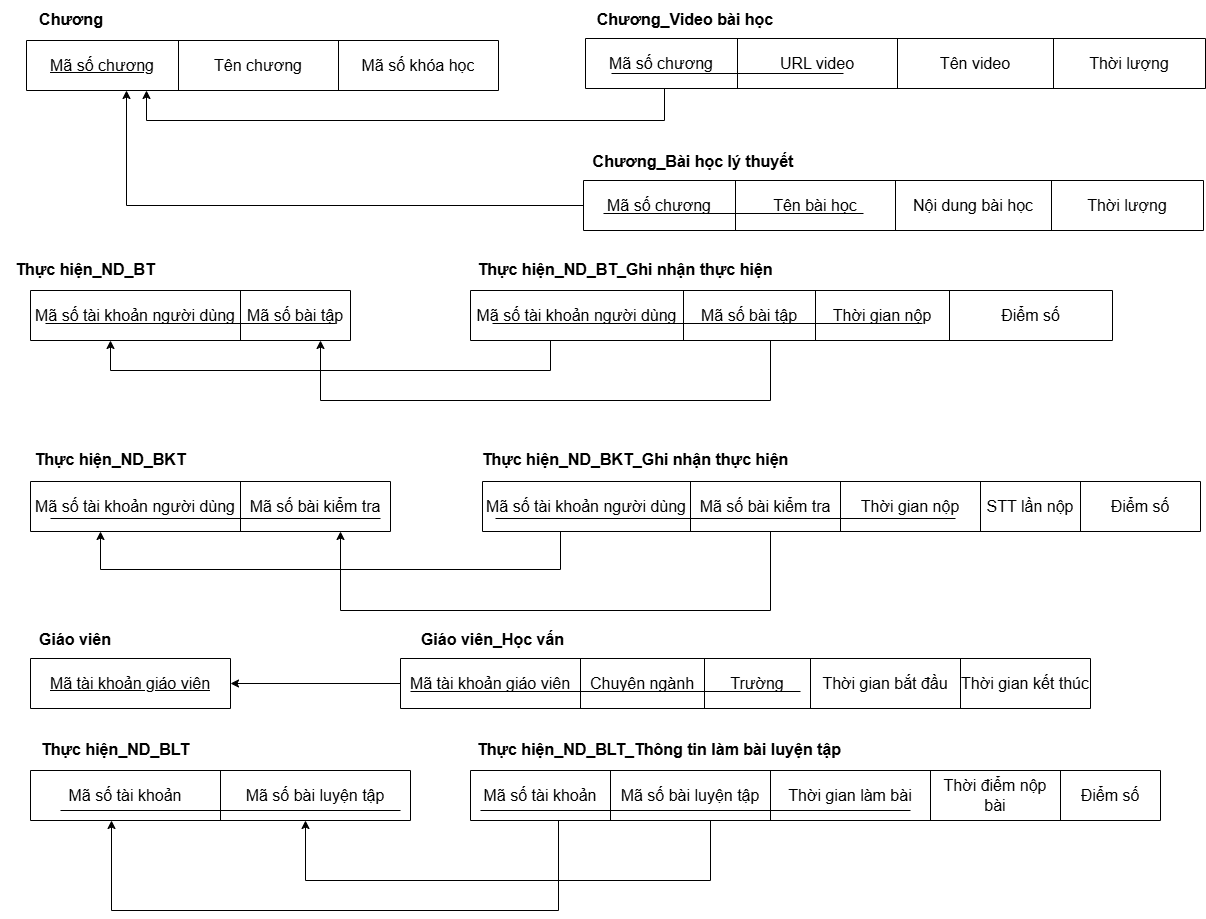
\includegraphics[width=1\linewidth]{picture/datri.png}
    \caption{Bước 6: Ánh xạ các thuộc tính đa trị (Multivalued	attributes)}
    \label{fig:placeholder}
\end{figure}
\subsection{Bước 7: Ánh xạ chuyên biệt hóa (lớp cha – lớp con)}
Lớp \textbf{NGƯỜI DÙNG} có lớp con là \textbf{GIÁO VIÊN}.
\begin{figure}[H]
    \centering
    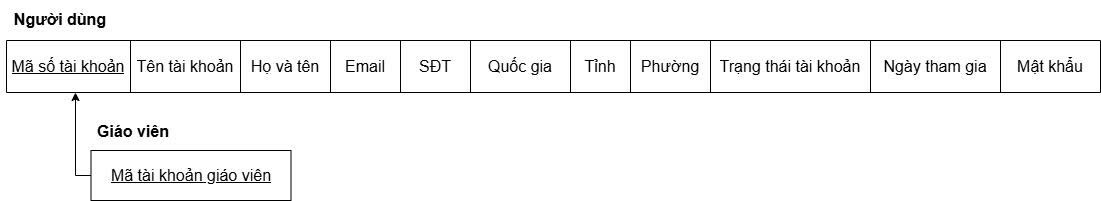
\includegraphics[width=1\linewidth]{picture/chacon.jpg}
    \caption{Bước 7: Ánh xạ chuyên biệt hóa (lớp cha – lớp con)}
    \label{fig:placeholder}
\end{figure}
\end{document}